\documentclass[nobib]{tufte-handout}

\title{Föreläsning 4: Sammanfattning av alla räkneproblem, samt cykler $\cdot$ 1MA020}

\author[Vilhelm Agdur]{Vilhelm Agdur\thanks{\href{mailto:vilhelm.agdur@math.uu.se}{\nolinkurl{vilhelm.agdur@math.uu.se}}}}

%\date{15 januari 2023}


%\geometry{showframe} % display margins for debugging page layout

\usepackage{graphicx} % allow embedded images
  \setkeys{Gin}{width=\linewidth,totalheight=\textheight,keepaspectratio}
  \graphicspath{{graphics/}} % set of paths to search for images
\usepackage{amsmath}  % extended mathematics
\usepackage{booktabs} % book-quality tables
\usepackage{units}    % non-stacked fractions and better unit spacing
\usepackage{multicol} % multiple column layout facilities
\usepackage{lipsum}   % filler text
\usepackage{fancyvrb} % extended verbatim environments
  \fvset{fontsize=\normalsize}% default font size for fancy-verbatim environments

\usepackage{color,soul} % Highlights for text

% Standardize command font styles and environments
\newcommand{\doccmd}[1]{\texttt{\textbackslash#1}}% command name -- adds backslash automatically
\newcommand{\docopt}[1]{\ensuremath{\langle}\textrm{\textit{#1}}\ensuremath{\rangle}}% optional command argument
\newcommand{\docarg}[1]{\textrm{\textit{#1}}}% (required) command argument
\newcommand{\docenv}[1]{\textsf{#1}}% environment name
\newcommand{\docpkg}[1]{\texttt{#1}}% package name
\newcommand{\doccls}[1]{\texttt{#1}}% document class name
\newcommand{\docclsopt}[1]{\texttt{#1}}% document class option name
\newenvironment{docspec}{\begin{quote}\noindent}{\end{quote}}% command specification environment

\include{mathcommands.extratex}

\begin{document}

\definecolor{darkgreen}{rgb}{0.0627, 0.4588, 0.1451}

\maketitle% this prints the handout title, author, and date

\begin{abstract}
\noindent
Vi fortsätter studera inklusion-exklusion, och ger fler tillämpningar.
\end{abstract}

\section{Surjektioner}

\begin{definition}
  Låt $A$ och $B$ vara två mängder, och $f: A \to B$ en funktion. Vi definierar \emph{bilden} av $A$ som
  $$f(A) = \left\{b \in B \given \exists a\in A: f(a) = b\right\},$$
  det vill säga alla element i $B$ som träffas av något element i $A$ under $f$.

  Funktionen $f$ är en \emph{surjektion} om $f(A) = B$. Om det finns en surjektion från $A$ till $B$ gäller det att $\abs{A} \geq \abs{B}$.\sidenote[][]{Detta är uppenbart för ändliga mängder $A$ och $B$ -- för oändliga mängder är detta definitionen av ordningen mellan kardinaltal.}
\end{definition}

\begin{definition}
  För $n \geq m \geq 1$ ges \emph{Stirlings partitionstal}, också kallat \emph{Stirlingtalet av andra sorten}, av
  $$\stirlingPart{n}{m} = \frac{1}{m!}\sum_{k=0}^{m}(-1)^k\binom{m}{k}(m-k)^n.$$
\end{definition}

\begin{theorem}\label{theorem_count_surjections}
  Låt $A$ och $B$ vara ändliga mängder med $\abs{A} = n$, $\abs{B} = m$, och $n \geq m$. Antalet surjektioner från $A$ till $B$ ges av
  $$S(n,m) = m!\stirlingPart{n}{m} = \sum_{k=0}^{m} (-1)^k \binom{m}{k}(m-k)^n.$$

  \begin{proof}
    Låt $X$ vara mängden av alla funktioner från $A$ till $B$, och för varje $b \in B$, låt $X_b$ vara mängden av funktioner från $A$ till $B$ som inte träffar $b$. Vi vill, som vanligt, räkna ut $\abs{X \setminus \bigcup_{b\in B} X_b} = \abs{X} - \abs{\bigcup_{b\in B} X_b}$.

    Multiplikationsprincipen ger oss enkelt att $\abs{X} = m^n$ -- varje element i $A$ har $m$ val för var det skall skickas, och vi har $n$ stycken element att göra det valet för.

    Inklusion-exklusion ger oss att
    $$\abs{\bigcup_{b\in B} X_b} = \sum_{I \subseteq B} (-1)^{\abs{I} + 1}\abs{\bigcap_{b \in I} X_b}$$
    och vad vi behöver räkna är antalet funktioner från $A$ till $B$ som undviker att träffa en viss mängd $I$. Ett specialfall ser vi omedelbart -- om $I = B$ måste snittet vara tomt, eftersom elementen i $A$ måste skickas \emph{någonstans}.

    Att räkna dem är relativt enkelt -- en funktion från $A$ till $B$ som inte träffar en viss mängd $I \subset B$ är ju precis en funktion från $A$ till $B \setminus I$, och vi vet att det finns $\abs{B \setminus I}^{\abs{A}} = (m - \abs{I})^n$ sådana. Så vad vi får är att
    $$\abs{\bigcup_{b\in B} X_b} = \sum_{I \subset B, I \neq B} (-1)^{\abs{I} + 1}(m - \abs{I})^n.$$

    Så om vi grupperar den här summan efter storleken på $I$ vet vi att det finns $\binom{m}{k}$ stycken val av $I$ av storlek $k$, så 
    $$\abs{\bigcup_{b\in B} X_b} = \sum_{k=0}^{m-1} (-1)^{k + 1}\binom{m}{k}(m - k)^n$$
    vilket ger oss resultatet, när vi stoppar in detta i $S(n,m) = \abs{X} - \abs{\bigcup_{b\in B} X_b}$.
  \end{proof}
\end{theorem}

\begin{example}
  Antag att en farmor stickat fem filtar åt sina tre barnbarn. På hur många sätt kan hon fördela filtarna, så att varje barn får åtminstone en filt? Eftersom de är handstickade är så klart filtarna \emph{särskiljbara}, så det här är inte ett exempel på de kompositioner vi såg i föreläsning två, utan ett exempel på surjektioner.

  Vår sats säger oss att svaret är $3!\stirlingPart{5}{3} = 150$.
\end{example}

\section{Mängdpartitioner}

Hur många sätt finns det att fördela $n$ objekt i $k$ stycken olika högar? Här har vi en ny variant på räkneproblem -- istället för att vi har objekt som är särskiljbara eller inte så har vi nu osärskiljbara \emph{lådor}.

\begin{theorem}
  Antag att vi har en mängd $X$ med $\abs{X} = n$. Ett sätt att dela upp denna mängd i $k$ osärskiljbara högar\sidenote[][]{Alltså, för den som vill vara formell, ett sätt att skriva $X = A_1 \cup A_2 \cup \ldots \cup A_k$ där $A_i \cap A_j = \emptyset$ för $i \neq j$, där etiketterna på våra $A_i$ inte spelar roll. Eller så kan man se det som en ekvivalensrelation på $X$ med $k$ delar.} kallas för en \emph{mängdpartition} av $X$ i $k$ delar.

  Antalet sådana ges av
  $$\stirlingPart{n}{k}.$$

  \begin{proof}
    Vi bevisar detta genom att räkna antalet surjektioner från $X$ till $[k]$ på två olika sätt.

    Beteckna antalet mängdpartitioner av $X$ i $k$ delar med $m$. Vi kan skapa oss en surjektion från $X$ till $[k]$ genom att först dela upp $X$ i $k$ delar, och sedan ge etiketter från $1$ till $k$ till delarna. Vår surjektion blir då att vi skickar del $i$ till talet $i \in [k]$. Eftersom det finns $k!$ sätt att tilldela etiketterna (etiketteringen är en permutation av längd $k$ från $[k]$) säger oss Multiplikationsprincipen att det måste finnas $k!m$ surjektioner från $X$ till $[k]$.

    Men vi vet också av Teorem \ref{theorem_count_surjections} att antalet surjektioner ges av $k!\stirlingPart{n}{k}$. Alltså måste $m = \stirlingPart{n}{k}$, som önskat.
  \end{proof}
\end{theorem}

\section{Den tolvfaldiga vägen}

När vi talade om kompositioner fördelade vi alltså osärskiljbara objekt i särskiljbara lådor -- och studerade både fallet där lådor fick vara tomma, och när de inte fick det. För surjektioner fördelar vi särskiljbara objekt i särskiljbara lådor, och kräver att varje låda får ett objekt.

Vi börjar ana ett mönster här i hur våra problem kan se ut. Vi kan ha
\begin{enumerate}
  \item Särskiljbara objekt och särskiljbara lådor
  \item Osärskiljbara objekt och särskiljbara lådor
  \item Särskiljbara objekt och osärskiljbara lådor
  \item Osärskiljbara objekt och osärskiljbara lådor
\end{enumerate}
och vi kan ha olika krav på hur objekten fördelas i lådorna
\begin{enumerate}
  \item Generell -- lådor får vara tomma och får innehålla hur många objekt som helst
  \item Surjektiv -- varje låda måste innehålla något objekt
  \item Injektiv -- ingen låda får innehålla mer än ett objekt
\end{enumerate}
så sammanfattningsvis har vi en tabell med tolv stycken tänkbara kombinatorikproblem. Det kommer visa sig att vi i själva verket redan studerat sju av dem.


Under föreläsning två pratade vi om fördelningar av osärskiljbara objekt mellan särskiljbara personer, och gav en formel för deras antal i Proposition 11, men vi gav aldrig ett kort namn åt detta problem. Låt oss kalla en sådan fördelning för en \emph{multi-delmängd} till mängden av personer.

En \emph{multi-mängd} är som en vanlig mängd, fast den får innehålla ett och samma objekt mer än en gång. Så vi betraktar alltså fördelningen av objekt mellan personer som en multi-delmängd genom att tänka att varje person är med i multidelmängden lika många gånger som antalet objekt den fick.

Så låt oss rita denna tabell -- problem vi redan studerat är i svart text, problem vi inte sett innan är i \textcolor{darkgreen}{grön text}. Låt $N$ vara en mängd av $n$ \emph{objekt}, och $X$ vara en mängd av $x$ \emph{lådor}. Vi ser fördelningarna av objekt i lådor som en funktion $f: N \to X$.

\begin{fullwidth}
  \begin{tabularx}{\linewidth}{l|ccc}
      & Generellt $f$ & Injektivt $f$ & Surjektivt $f$\\
      \midrule
    Bägge särskiljbara & \specialcell{Ord ur $X$ av längd $n$\\ $x^n$} & \specialcell{Permutation ur $X$ av längd $n$\\ $\frac{x!}{(x-n)!}$} & \specialcell{Surjektion från $N$ till $X$\\$x!\stirlingPart{n}{x}$} \\
    Osärskiljbara objekt & \specialcell{Multi-delmängd av $X$\\ av storlek $n$\\$\binom{n + x - 1}{n}$} & \specialcell{Delmängd av $X$ av storlek $n$\\$\binom{x}{n}$} & \specialcell{Kompositioner av $n$\\av längd $x$\\$\binom{n - 1}{n - x}$} \\
    Osärskiljbara lådor & \specialcell{\textcolor{darkgreen}{Mängdpartition av $X$}\\ \textcolor{darkgreen}{ i $\leq x$ delar} \\\textcolor{darkgreen}{$\sum_{k=1}^{x} \stirlingPart{n}{k}$}} & \specialcell{\textcolor{darkgreen}{Mängdpartition av $X$}\\ \textcolor{darkgreen}{i $\leq x$ delar av storlek $1$}\\\textcolor{darkgreen}{$1$ om $n \leq x$, $0$ annars}} & \specialcell{Mängdpartition av $N$\\i $x$ delar\\$\stirlingPart{n}{x}$} \\
    Bägge osärskiljbara & \specialcell{\textcolor{darkgreen}{Heltalspartition av $n$ i $\leq x$ delar}\\\textcolor{darkgreen}{$p_x(n + x)$}} & \specialcell{\textcolor{darkgreen}{Sätt att skriva $n$ som}\\\textcolor{darkgreen}{summan av $\leq x$ ettor}\\\textcolor{darkgreen}{$1$ om $n \leq x$, $0$ annars}} & \specialcell{\textcolor{darkgreen}{Heltalspartitioner av $n$}\\ \textcolor{darkgreen}{i $x$ delar} \\\textcolor{darkgreen}{$p_x(n)$}} 
  \end{tabularx}
\end{fullwidth}

\section{Stirlingtalen av första sorten}

I början av denna föreläsningen introducerade vi Stirlingtalen av \emph{andra} sorten, vilket ju leder en till att fråga vad den första sorten är. Så låt oss introducera ett problem till vilket dem är lösningen:

\begin{definition}
  Antag att $n$ personer skall sitta runt $k$ stycken osärskiljbara runda bord, och varje bord måste ha minst en person som sitter vid det. Då ges antalet sätt att placera personerna runt borden av $\stirlingCycle{n}{k}$, \emph{Stirlings cykeltal}. Stirlings cykeltal kallas också för \emph{Stirlingtalen av första sorten}.
\end{definition}

Till skillnad från Stirlings partitionstal finns det inte någon enkel formel för cykeltalen. Vi kan däremot bevisa följande resultat:

\begin{theorem}
  Det gäller, för alla $n \geq 1$, att
  $$\sum_{k=1}^{n} \stirlingCycle{n}{k} = n!.$$

  \begin{proof}
    Vi bevisar detta genom att uppvisa en bijektion mellan mängden av permutationer av längd $n$ ur $[n]$, vilka vi vet att det finns $n!$ av, och samlingen av sätt att placera personer runt ett godtyckligt antal runda bord, vilka vi vet per definition räknas av $\sum_{k=1}^{n} \stirlingCycle{n}{k}$.

    \begin{marginfigure}\label{fig_cycles_of_permutation}
      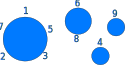
\includegraphics{graphics/cycles_of_permutation.pdf}
      \caption{Ett exempel på ett sätt placera nio personer vid runda bord. Den motsvarande permutationen till detta sätt att placera personer är $572438169$. Det vanliga sättet att skriva detta sätt att placera personer vid bord i text är $(15327)(4)(68)(9)$.}
    \end{marginfigure}

    Givet ett sätt att placera $n$ personer runt något antal runda bord kan vi definiera en permutation $\sigma$ genom att, på plats $i$ i permutationen, skriva den person som sitter till vänster om person $i$ runt deras bord. (En person som sitter ensam anser vi sitta till vänster om sig själv.) Detta kommer ge oss en permutation eftersom varje person bara har en person till höger om sig, så ingen person kommer dyka upp två gånger, och varje person har bara en person till vänster om sig, så $\sigma(i)$ är väldefinierat för varje $i$.

    Givet en permutation $\sigma$ kan vi placera ut personer runt runda bord som följer: Vi börjar med att ställa fram ett bord, och sätta person ett vid det bordet. Sedan sätter vi person $\sigma(1)$ till vänster om person ett, och person $\sigma(\sigma(1))$ till vänster om person $\sigma(1)$, och så vidare. Förr eller senare måste vi komma tillbaka till person $1$, eftersom det bara finns ändligt många personer. Om vi placerat alla personerna runt vårt första bord är vi klara.

    Om vi har några personer kvar att placera plockar vi fram ett till bord, och sätter den person med lägst nummer som inte redan har en sittplats vid det bordet -- säg att det är person $j$. Sedan upprepar vi processen från innan, och placerar person $\sigma(j)$ till vänster om henne, person $\sigma(\sigma(j))$ till vänster om person $\sigma(j)$, och så vidare. Återigen kommer vi förr eller senare komma tillbaka till person $k$, och ha gått full cirkel.

    Vi upprepar denna process med fler bord ända tills varje person har fått ett bord, och vi har fått oss ett sätt att placera $n$ personer runt något antal bord mellan $1$ och $n$.

    Det är någorlunda enkelt att se, efter att man funderat en stund, att vi alltid kommer komma tillbaka till samma permutation vi började med om vi först skapar en bordsplacering av permutationen, och sedan skapar en permutation av den bordsplaceringen. Alltså är detta en bijektion, och vi har bevisat vår formel.
  \end{proof}
\end{theorem}

\begin{remark}
  Vi har introducerat detta som ``personer runt runda bord'', men den vanliga matematiska terminologin runt detta är ``cykler i en permutation''. Hittills har vi bara sett permutationer som en lista av tal i någon ordning, där varje tal mellan $1$ och $n$ dyker upp exakt en gång, men detta är bara ett perspektiv på vad en permutation är.

  Perspektivet med cykler är ett minst lika vanligt perspektiv på permutationer, och framhäver andra saker man kan använda dem för. För att representera dessa i text skriver vi vanligen i formatet $(15327)(4)(68)(9)$, såsom i Figur \ref{fig_cycles_of_permutation}, i stället för att rita cirklar med tal runt dem.
\end{remark}

\section{Övningar}

\begin{xca}
  Ge ett kombinatoriskt bevis för att
  $$\stirlingPart{n}{k} = k\stirlingPart{n-1}{k} + \stirlingPart{n-1}{k-1}.$$
\end{xca}

\begin{xca}
  Ge kombinatoriska bevis för att
  $$\stirlingPart{n}{n-1} = \binom{n}{2}$$
  och
  $$\stirlingPart{n}{2} = 2^{n-1} - 1.$$
\end{xca}

\begin{xca}
  Ge ett kombinatoriskt bevis för att
  $$\stirlingPart{n+1}{k} = \stirlingPart{n}{k-1} + n\stirlingPart{n}{k}.$$
\end{xca}

%\bibliography{references}
%\bibliographystyle{plainnat}

\end{document}
